\documentclass[a4paper,dvipdfmx]{jsarticle}
\usepackage{graphicx}
\usepackage{fancybox}
\usepackage{ascmac}
\usepackage{amsmath}
\usepackage{amsfonts}
\usepackage{comment}
\usepackage{here}
\usepackage{listings,jlisting}
\usepackage[a4paper,margin=2cm,truedimen]{geometry}
\usepackage{amssymb}
\usepackage[svgnames]{xcolor}

  \definecolor{diffstart}{named}{Grey}
  \definecolor{diffincl}{named}{Green}
  \definecolor{diffrem}{named}{OrangeRed}

  \lstdefinelanguage{diff}{
    basicstyle=\ttfamily\small,
    morecomment=[f][\color{diffstart}]{@@},
    morecomment=[f][\color{diffincl}]{+\ },
    morecomment=[f][\color{diffrem}]{-\ },
  }

\newcommand{\image}[2]{
    \begin{figure}[H]
        \begin{center}
        \includegraphics[width=14cm]{#2}
        \end{center}
        \caption{#1}
        \label{#1}
    \end{figure}
}

\lstset{
	%language=[Objective]Caml,
	language=Python,
    basicstyle=\ttfamily,
    keywordstyle=\color[RGB]{33,74,135}\bfseries,
    stringstyle=\color[RGB]{79,153,5},
    commentstyle=\color[RGB]{143,89,2}\itshape,
    numberstyle=\footnotesize,
    numbers=left,
    stepnumber=1,
    numbersep=15pt,
    backgroundcolor=\color[RGB]{251,251,251},
    frame=single,
    frameround=ffff,
    framesep=5pt,
    rulecolor=\color[RGB]{148,150,152}, 
    breaklines=true,
    breakautoindent=true,
    breakatwhitespace=true,
    breakindent=25pt,
    showspaces=false,
    showstringspaces=false,
    showtabs=false,
    tabsize=2,
    captionpos=b,
    linewidth=\textwidth,
}
%\end{comment}
\begin{document}
% タイトルはここ
%\title{機能設計仕様書}
% 自分の情報はここに
%\author{工学部情報学科計算機科学コース \\ 1029-28-8969 渡邊 綾仁}

% 提出日って書いているけどコンパイルした日
% 使いたくなかったらコメントアウト

% \date{提出日: \today}

%\maketitle

% 以下、コピペ用
% includegraphicsとかtableとかめんどくさいのでここに書いておくとよさそう

\begin{comment}
%コメントアウトここから
% ----------------

%画像挿入用
\begin{figure}[H]
\begin{center}
\includegraphics[width=14cm]{hoge.png}
\end{center}
\caption{キャプション}
\label{参照ラベル}
\end{figure}

%ソースコード挿入用
\begin{lstlisting}[basicstyle=\ttfamily\footnotesize, frame=single]
\end{lstlisting}

%table環境
\begin{table}[H]
\begin{center}
\caption{キャプション}
  \begin{tabular}{|c|c|c|c|} \hline
    ノード名 & 割り当てたピンの番号 & 信号名 & スイッチ名 \\ \hline \hline
  \end{tabular}
	\label{ラベル}
\end{center}
\end{table}


%コメントアウトおしまい
\end{comment}

%20180506 メモ
\begin{comment}
simple.pdfのSIMPLE/Bの記述が、方式設計レベルの仕様書に該当するようなので、
このような記述方法を参考にすると、多分system_design_spec.pdfは書きやすいかも。
\end{comment}
%メモおしまい

% ----------------
%ここから本文

\section*{発展課題の実装内容}

以下、ソースコードについて、関数やクラスのコメント部分については省略している。

\subsection*{A1: ReLU}

\subsubsection*{実装内容}

ReLU 関数の順伝播の定義は my\_nn\_learn.py 内にあり、以下のソースコード \ref{A1-1} のようになっている。

\begin{lstlisting}[caption="ReLU 関数(順伝播)",label=A1-1]
def relu_forward(t: ndarray) -> ndarray:
    return np.maximum(t, 0)
\end{lstlisting}

また、ReLU の逆伝播を行う関数については以下のソースコード \ref{A1-2} のようになっている。

\begin{lstlisting}[caption="ReLU 関数(逆伝播)",label=A1-2]
def relu_backward(t: ndarray) -> ndarray:
    return np.where(t > 0, 1, 0)
\end{lstlisting}

必須課題においては中間層の活性化関数にシグモイド関数を用いていたが、この活性化関数を ReLU 関数に置き換えた。また、逆伝播についても、シグモイド関数の微分ではなく、ReLU 関数の微分に置き換えた。変更内容はソースコード \ref{A1-3} のようになっている。

\begin{lstlisting}[caption="中間層の変更内容",label=A1-3]
def mid_layer_activation(t: ndarray) -> ndarray:
    # return np.apply_along_axis(f_sigmoid, axis=0, arr=t)
    return np.apply_along_axis(relu_forward, axis=0, arr=t)

...

def back_prop(nn: NNLearn, data: dict):
...
    # 3. back propagate : sigmoid
    # sigmoid function ver.
    # bp_sigmoid = np.dot(nn.network['w2'].T, grad_en_ak) * (1 - f_sigmoid(data['a1'])) * f_sigmoid(data['a1'])

    # relu function ver.
    bp_sigmoid = np.dot(nn.network['w2'].T, grad_en_ak) * relu_backward(data['a1'])
\end{lstlisting}

ソースコード \ref{A1-3} の 3 行目が順伝播において活性化関数に ReLU 関数を適用する部分、14 行目が逆伝播を行っている部分に相当する。

\subsubsection*{実行結果}

バッチサイズ $100$、学習係数 $0.01$、エポック数 $10$ にして横軸に学習回数、縦軸にクロスエントロピー誤差の平均値をとったグラフを作成したところ、以下の図 \ref{fig-A-1-1} のようになった。

\begin{figure}[H]
\centering
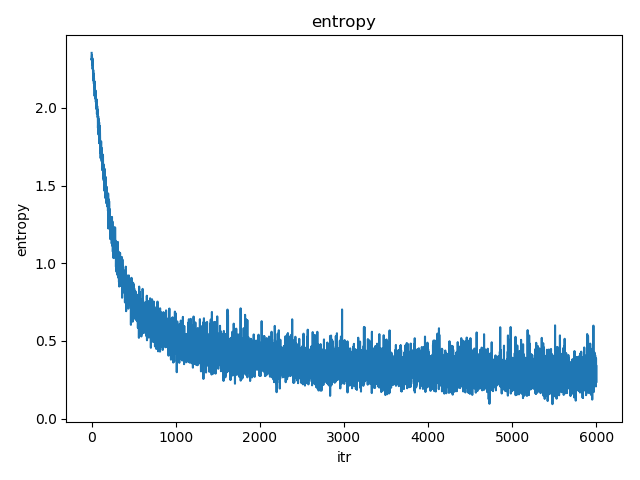
\includegraphics[width=12cm]{report_ReLU10epoch.png}
\caption{学習の経過}
\label{fig-A-1-1}
\end{figure}

図 \ref{fig-A-1-1} から、学習が正しく進んでいると考えられる。

\subsection*{A2: Dropout}

\subsection*{A4-1: 最適化手法の改良...Momentum SGD}


\subsection*{A4-2: 最適化手法の改良...AdaGrad}

\subsection*{A4-3: 最適化手法の改良...RMSProp}

\subsection*{A4-4: 最適化手法の改良...AdaDelta}

\subsection*{A4-5: 最適化手法の改良...Adam}

\subsection*{A5: カラー画像への拡張}

\subsubsection*{実装内容}

新たにカラー画像の学習用のプログラムファイル my\_nn\_color\_learn.py とテスト用プログラムファイル my\_nn\_color\_test.py を用意した。実装内容は以下の通りである。

\begin{itemize}
	\item モノクロ画像では Python3 系で学習させていたが、cPickle を用いるため Python2 系で実装を行った
	\item 次元数を $ d=1 \times 28 \times 28 $ から $ d=3 \times 32 \times 32 $ に変更
	\item 中間層のノード数を 1000 に変更
	\item 中間層の活性化関数は ReLU
	\item 逆伝播後の最適化手法は Adam を採用
	\item Adam のパラメータは $\alpha = 0.001, \beta_1 = 0.9, \beta_2 =  0.999, \epsilon = 10^{-8}$ に設定
\end{itemize}

\end{document}
